\chapter{OVERALL DESCRIPTION}
\label{ch:overallDescription}%
% The \label{...}% enables to remove the small indentation that is generated, always leave the % symbol.

\section{Product Perspective}
\label{sec:productPerspective}

\subsection{Scenarios} %AS
\label{subsec:scenarios}
\begin{enumerate}
\item \textbf{Driver Registration}\\
Paolino is a professor in Milan and decides to start using the eMSP application just published by his students on the app store.
He downloads the app and then starts the signup process. The system asks him to insert various information about his personal data. Paolino fills all the text boxes and clicks confirm. The system then asks him for a valid payment method. After inserting it, a pop-up appears confirming its validity and finally, he receives a confirmation email from eMSP to conclude the registration. The system shows Paolino that the registration has been completed.
\item \textbf{Check nearby charging stations}\\
Franco is going on a trip with his new electric car and wants to take a break. Since he would have had to stop at a charging station in any case, he wants to take advantage of this break and charge his car so he can get to the destination with no more stops.
Franco, already registered to the eMSP, opens the application on his device, so he can check for charging stations in the selected area. 
Since Franco has planned to rest no more than half an hour, he selects from the eMSP application “Fast-charge” and gets a view of the map containing the charging stations supporting that charge type.
\item \textbf{Booking of a charge}\\
Renato needs to have a completely charged car for a work trip abroad after the weekend. He opens the eMSP application on his phone to check the map of nearby charging stations. He then chooses one station supporting the "Slow Charge", since he is not in a rush. After selecting it, the application shows the selected station page, containing the price per kWh and if existing, the corresponding offer, for the selected charging type. Since the station is not yet available, the app shows the remaining time before it is freed, which amounts to 60 minutes. As soon as the station becomes available he presses the “Book charge” button and selects the time of arrival. After receiving the notification that the booking was successful, along with the ID of the booked charging socket, Renato gets in his car and starts driving to the station.
\item \textbf{Car charging}\\
It’s 16:45 and Maristella has booked a charge for 17:00 for her truck. She arrives in time, parks her majestic truck and plugs in the charging cable to the charging socket. Finally, she presses the “Start charging” button displayed in the eMSP application on her device and starts the charging process. Her device now shows the estimated time until the recharge completes; meanwhile, Maristella decides to go to the station’s bar nearby for having her tea time. 
She’s having a good time when she suddenly remembers her dating invite.
Maristella takes her phone, opens the eMSP application and presses the “Stop charging” button; finally she receives a notification telling her that the payment was successful, so Maristella goes back to the charging station, unplugs the car and leaves happily with her truck.
\item \textbf{Receiving a charging Suggestion/Advice}\\
Cinzia is a professor in the province of Rome. She has been using the eMSP application for a while and has already authorized the system to read data about her calendar and her vehicle information such as navigation routes, location, and battery status. In the afternoon she has a meeting with one of her students to discuss about a very important project.  During lunchtime, she receives a notification on her phone from the eMSP application, saying that there is a personalized suggestion for her. She clicks on the notification, which opens the suggested station info page. She notices that it's on her route to the school and has set an offer for the fast-charge sockets. Since her car's battery level is at 20\% she decides to take advantage of the offer and starts the booking procedure.
\item \textbf{Applying offers for the charging prices}\\
Irene is employed by Be-Charge, a well-known CPO. She manages charging stations in the province of Naples and she decides to set a special offer to attract possible new customers in the newcome charging station that opened last week.
She logs in to the CPMS installed on her company computer and selects one of these charging stations. She then clicks on the “Set a new offer” button. The application asks her to fill out a form where she has to select the amount of discount and for which charging types and the expiration date for this offer. She sets a 10\% discount for all the available charging types and sets the expiration date to 7 days from that moment and finally clicks on the “Submit” button. She repeats this procedure for the other new charging stations and then logs out of the application.
\item \textbf{Update energy criteria}\\
Alice realizes that during the upcoming holidays a high percentage of the population will probably make road trips. She deduces that her charging stations will experience an increase in the number of customers. In order to withstand the high amount of energy that the charging stations will need to supply, she decides to update the criteria used by the CPMS to select the energy provider. She logs into the system and selects one of the most used stations. On its information page, she selects the "Update energy criteria" button. The system then shows the page with a form containing the available criteria. She chooses that the system will select the cheapest provider with enough capacity to power all sockets at full power and updates the revenue percentage for the energy sales from 10\% to 15\%. She then selects the "Update" button and waits for the system to send a confirmation. After repeating this procedure for all the charging stations that she expects will experience an increased influx, she logs out.
\item \textbf{Add a new charging station}\\
Francesco is working in his office when he receives an e-mail from his supervisor stating that the construction of two more charging stations in Pavia has just finished and they need to be added to the system. Therefore he logs into the CPMS application and selects the “Add charging station” button. The application opens a prompt asking him to select the station from the list of detected ones and he selects one of the two. The application then shows a form asking for the new charging station information, such as name, location and number of sockets. After inserting them, he clicks the "Submit" button. He is then redirected to the energy criteria page, where he only sets the revenue percentage for the energy sales to 10\%, leaving other fields empty. After receiving a confirmation notification he repeats the process for the other station and finally sends an e-mail to his supervisor to inform him that the task has been completed.

\end{enumerate}
The previously presented scenarios are the ones regarding the description of the sub-systems of this document. In order to clarify how the CPO can retrieve his credentials to access the CPMS and use it, another scenario is introduced. This scenario does \textbf{not} belong to the scope of this document.
\begin{enumerate}
    \setcounter{enumi}{8}
    \item \textbf{CPO registration}\\
    Marta just started a new company of charging stations in Foggia. In order to increase its number of customers, she decides to start using the eMall platform. She searches for eMall on her favourite search engine and, once found, she clicks on its website and then on "Register as CPO".
    The system asks her to insert various information about the organization and then checks its validity. She then receives a confirmation email with a download link to the CPMS software and the credentials to log in. She downloads the software and installs it.
\end{enumerate}
\subsection{Class Diagram}
\label{subsec:classDiagram}
    \begin{figure}[H]
        \begin{center}
        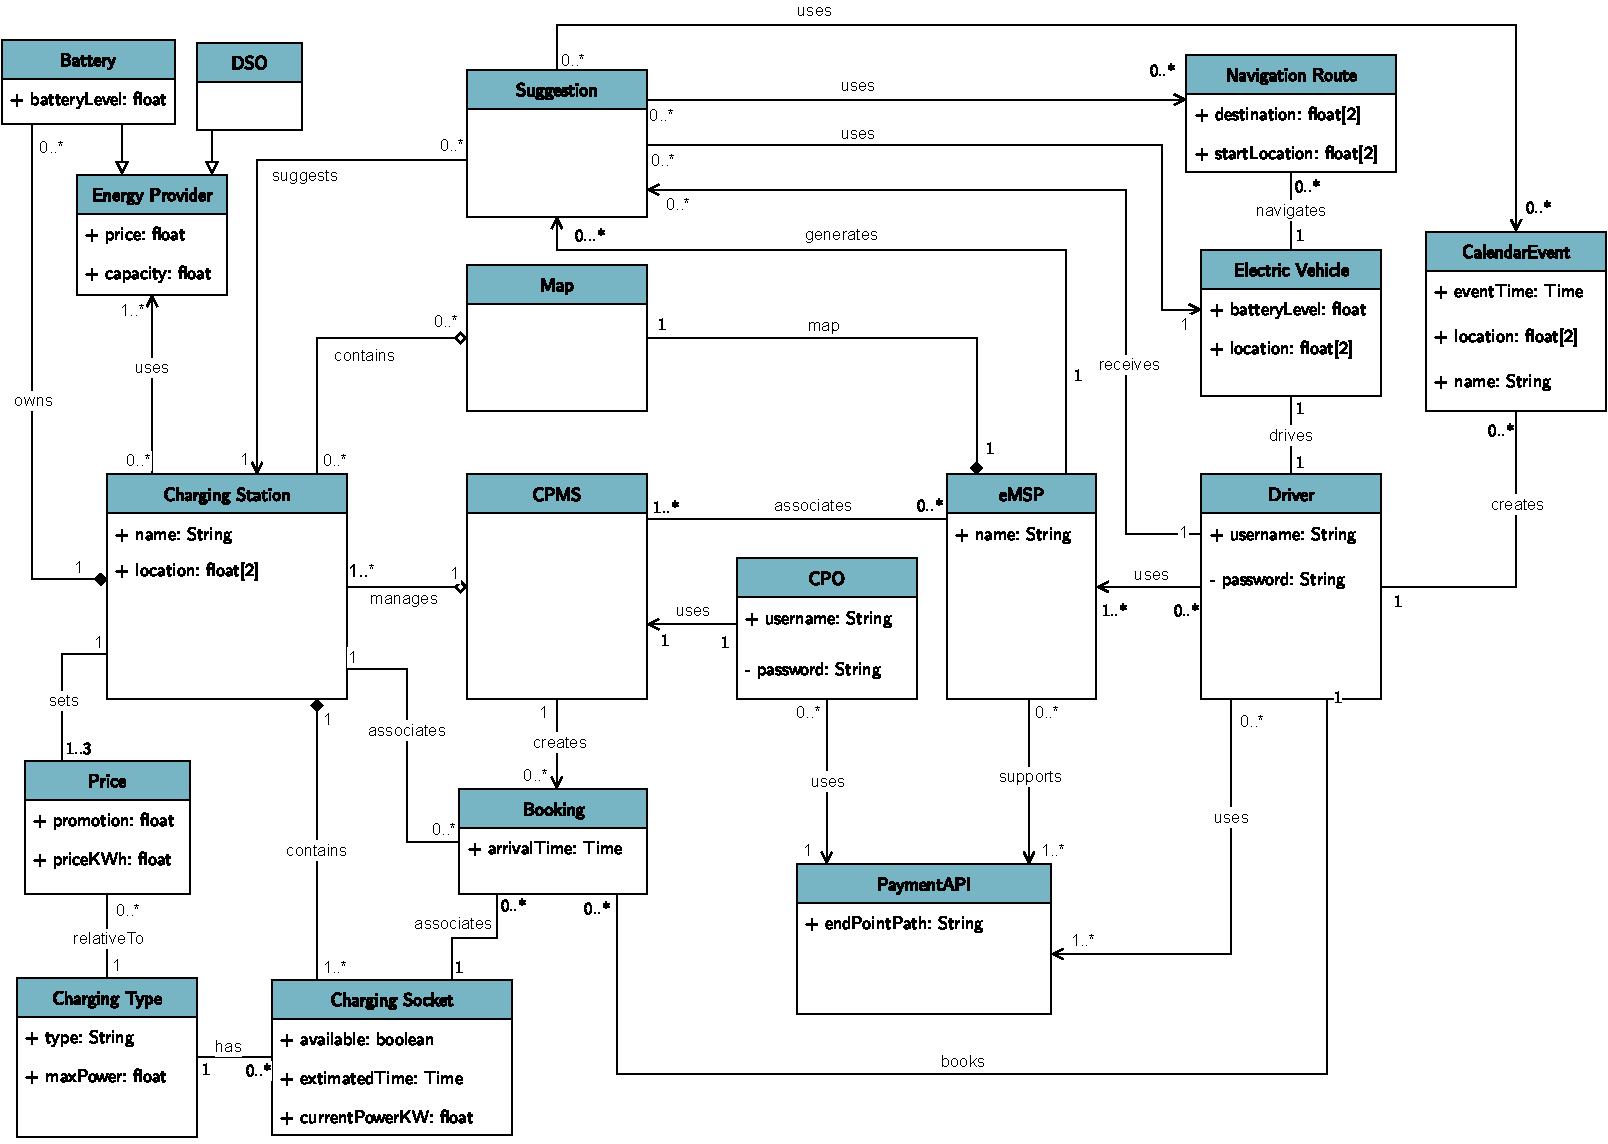
\includegraphics[
            width=\textwidth,
            height=\textheight,
            keepaspectratio]{classDiagram2}
        \caption{Class Diagram}
        \label{fig:classDiagram}
        \end{center}
    \end{figure}
    In this class diagram:
    \begin{itemize}
        \item Locations are represented with an array of 2 floats representing latitudes and longitudes.
        \item The Time type is used to represent a timestamp.
        \item The endPointPath attribute of the PaymentAPI class represents the URL from where the API sends requests.
    \end{itemize}     
    \newpage
\subsection{Dynamic Class Behaviour Models}
\label{subsec:statecharts}
The state diagrams listed below show the behaviour of the eMSP and the CPMS applications in their entirety.
\begin{itemize}
    \item \textbf{eMSP}
        \begin{figure}[H]
            \begin{center}
            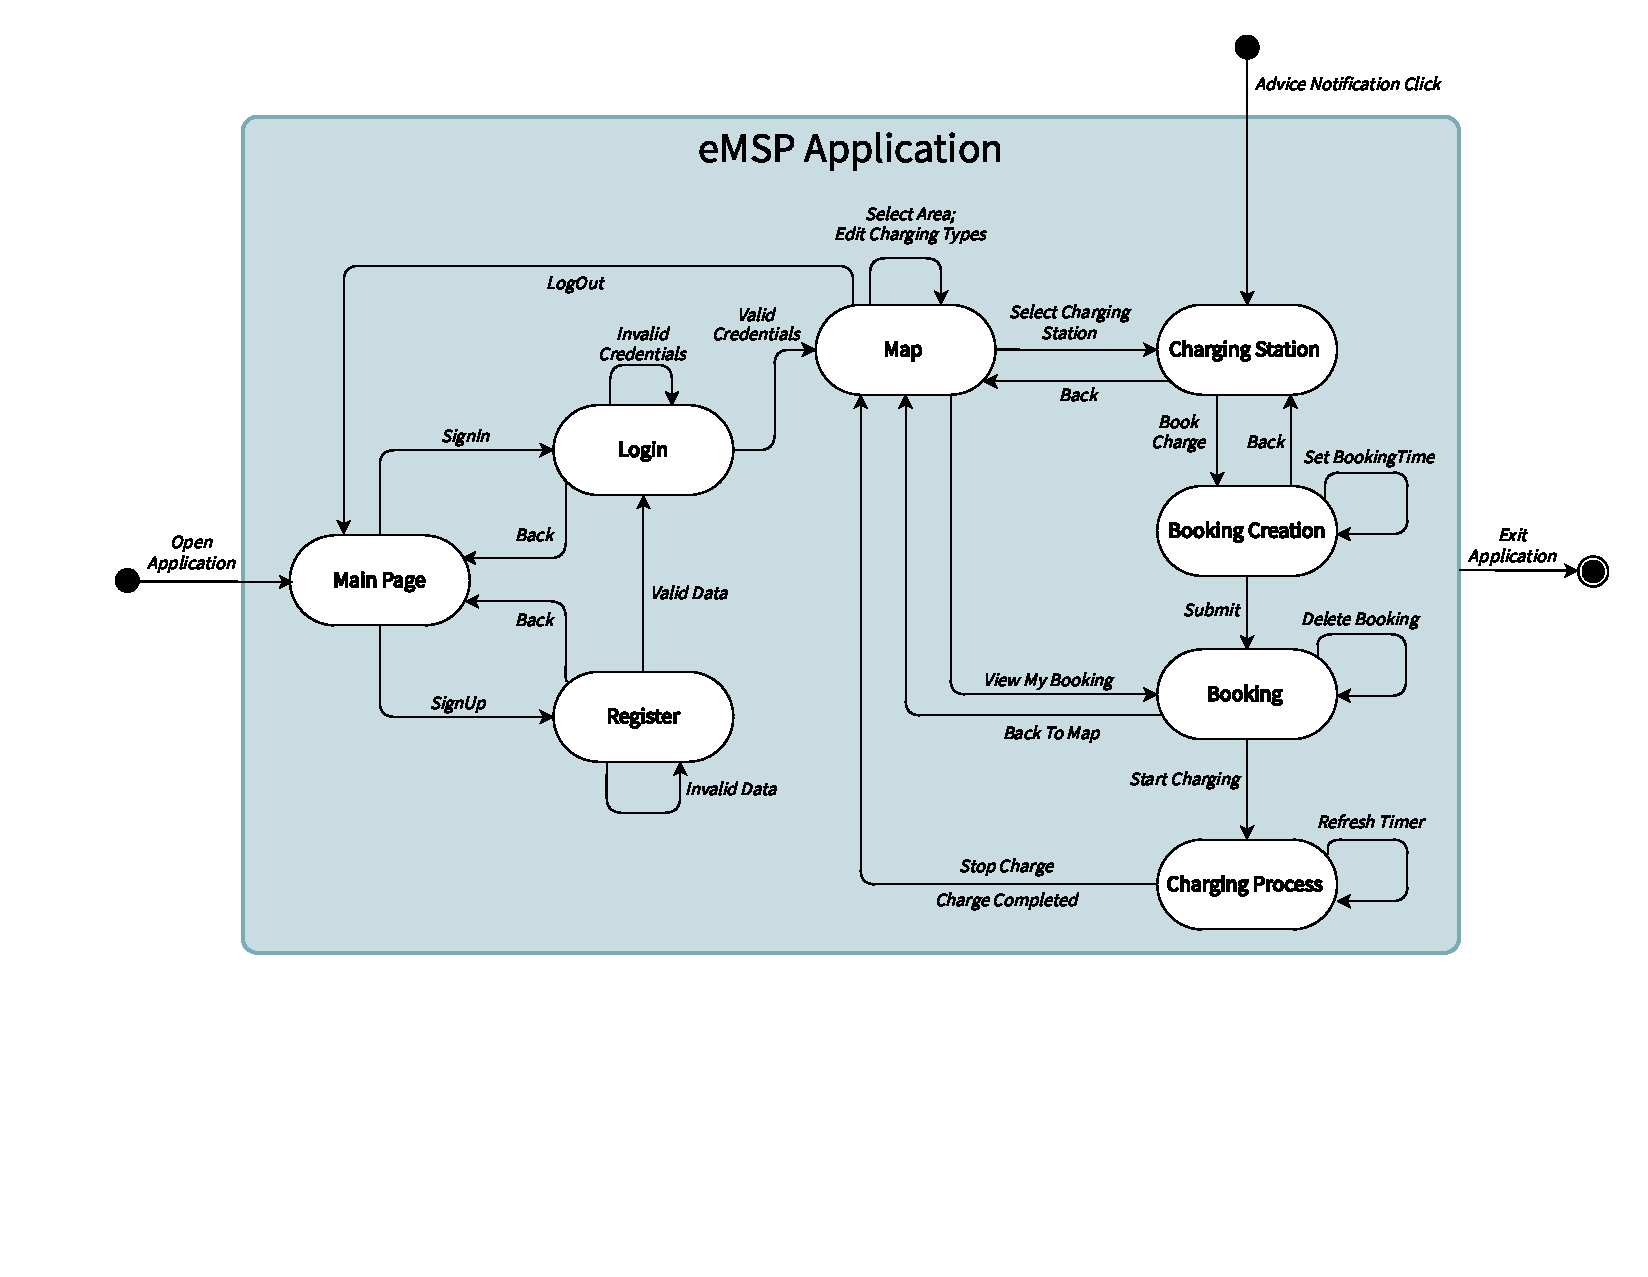
\includegraphics[
                width=\textwidth,
                height=\textheight,
                keepaspectratio]{StateCharts/eMSP}
            \caption{eMSP state diagram}
            \label{fig:eMSP}
            \end{center}
        \end{figure}
        \newpage
    \item \textbf{CPMS}
        \begin{figure}[H]
            \begin{center}
            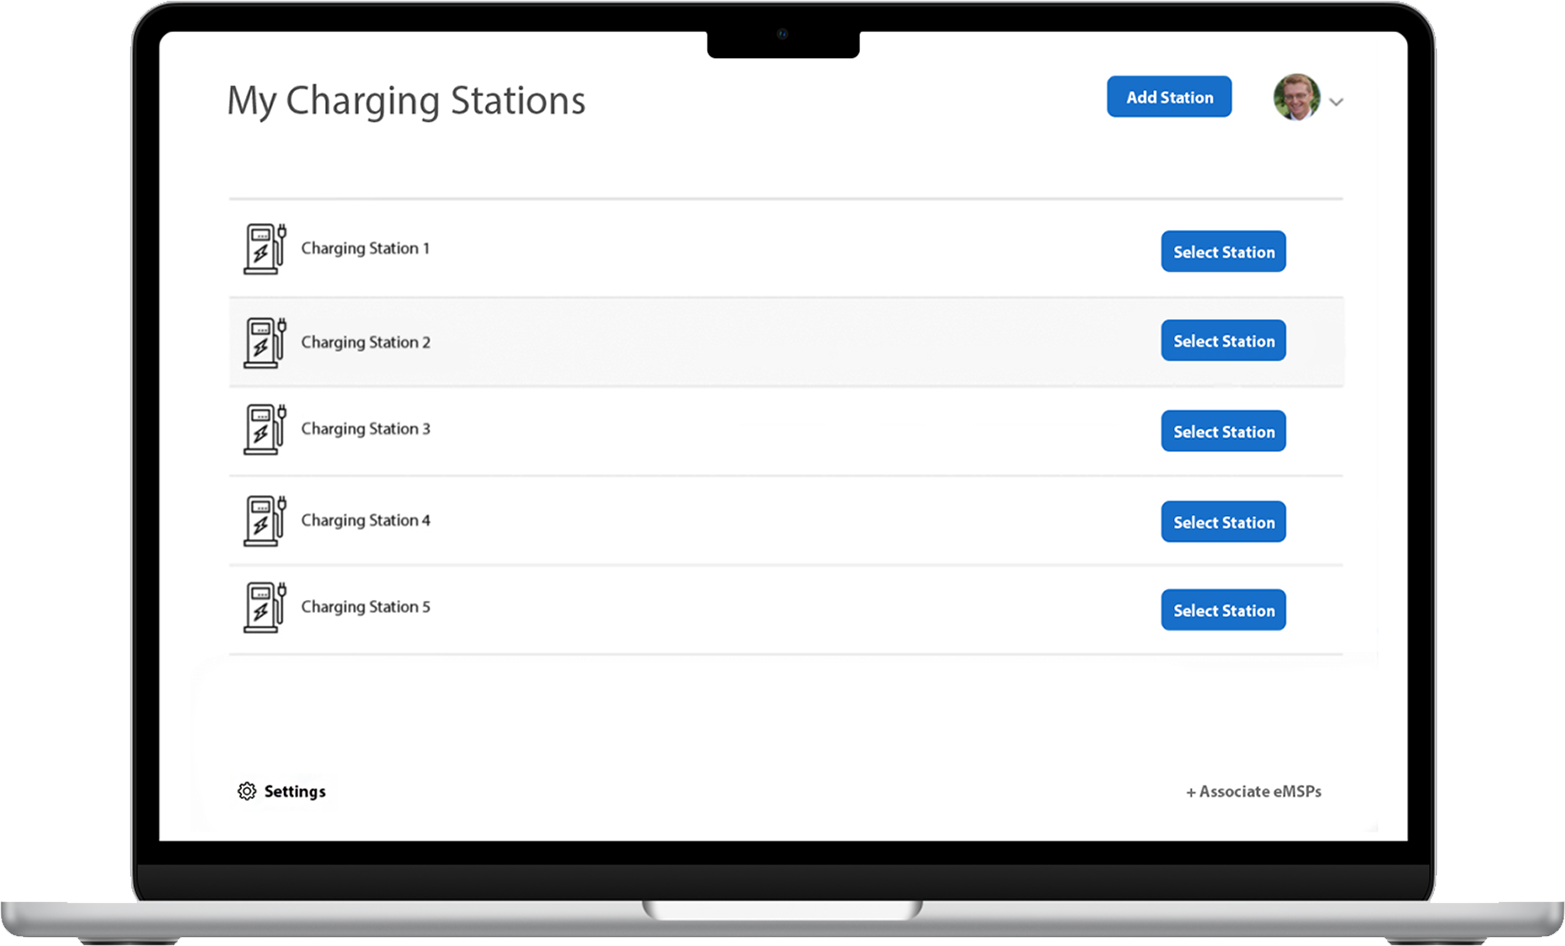
\includegraphics[
                width=\textwidth,
                height=\textheight,
                keepaspectratio]{StateCharts/CPMS}
            \caption{CPMS state diagram}
            \label{fig:CPMS}
            \end{center}
        \end{figure}
\end{itemize}
\section{Product Functions} %AP
\label{sec:productFunctions}
In this section, the main functionalities of our system are presented and described in more detail. \\
\textbf{Functionalities offered to the drivers through the eMSP:}
\begin{itemize}
    \item \textbf{Check charging stations in the surrounding area:} 
    The driver can check nearby charging stations through a map of available ones. They have the possibility to select a specific station, in order to get more details about it, such as its availability, the charging price and any active offers.
    \item \textbf{Book a charge:} The driver can book a charge at a specific station up to a maximum amount of time in advance, through the details page of said station. They can select the type of charging socket, if available, that they want to use to charge the vehicle.
    \item \textbf{Start the charging process:} The driver, once they have driven to the charging station they booked in advance, can initiate the charging process through the application. If the vehicle is not well connected to the socket, the application will send a notification to the driver.
    \item \textbf{Proactive charge suggestion:} The driver can receive a suggestion to charge their vehicle based on their schedule and route to their destination. The system will evaluate the charging stations near the driver's route and if the prices are advantageous and the charging can fit into their schedule it will send a suggestion to the driver through the application.
\end{itemize}
\textbf{Functionalities offered to the CPOs through the CPMSs:}
\begin{itemize}
    \item \textbf{Charging Stations Management:} The CPO is able to manage all his charging stations: he can decide with which eMSPs to associate his CPMS and which charging stations will be managed by it.\\
    For those charging stations, the system will automatically handle the energy acquisition following the criteria set by the CPO, for example, based on the energy providers' prices, and their maximum power delivery capacity.\\
    For all the charging stations connected to the CPMS, the CPO will be able to set special offers for the charging prices and to visualize info about their internal status, such as the amount of energy available for the batteries, if available, the number of vehicles being charged and, for each charging vehicle, they can see the amount of power absorbed. 
    %\item \textbf{Check status of charging station:} The CPO can check through the application all the details about the managed charging stations, such as the amount of energy available for the batteries, if available, the number of vehicles being charged and, for each charging vehicle, they can see the amount of power absorbed.
    %\item \textbf{Decide where to buy energy:} The CPO can check a list of all available DSOs and decide which one to buy the energy from. This functionality can also be fully automated by the CPMS, if desired.
    %\item \textbf{Set a promotion for the charging price:} The CPO has the possibility to create an offer for any number of charging stations managed and, for each charging type, possibly set a different discount to the relative price. In this way, they can strategically reduce any price in order to attract more customers. 
    %\item \textbf{Select energy acquisition criteria:} The CPO has the possibility to decide which criteria the system has to follow while deciding which energy provider to acquire energy from. These criteria comprise the cost of the provider and/or its maximum capacity.
    %\item \textbf{Add a new charging station:} The CPO has the possibility to add a new charging station to the ones managed by his CPMS.
    %\item \textbf{eMSP association:} The CPO has the possibility to associate his CPMS to any existing eMSP in order to keep it updated about all his managed charging stations.
    %\item \textbf{Energy storage management:} The CPO can decide to store any additional energy bought from a DSO to the charging station's batteries, if available. Moreover, they can decide whether to utilize the batteries or the DSO as the source of energy to power the charging sockets. This functionality can also be fully automated by the CPMS, if desired.
\end{itemize}

\section{User Characteristics} %AS
The system can be exploited by the following actors:
\label{sec:userCharacteristics}
\begin{enumerate}
\item \textbf{Unregistered Driver}\\
A driver who needs to register to the eMSP platform before being able to use any of its functionalities.
\item \textbf{Driver}\\
A driver that is registered on the eMSP platform and can use all its functionalities.
\item \textbf{CPO}\\
A CPO registered on eMall who can use all the functionalities offered by its CMPS.
\end{enumerate}

\newpage
\section{Assumptions, Dependencies and Constraints}
\label{sec:assumptionsDependenciesConstraints}

\subsection{Domain Assumptions} %AS
\label{subsec:domainAssumptions}
    \begin{longtable}{| p{0.15\linewidth} | p{0.8\linewidth} |}
    \hline
    \rowcolor{bluepoli!40}
     \textbf{ID} & \textbf{Description} \T\B \\
    \hline \hline
    \textbf{D\row} & The Driver's vehicle is electric and has a battery able to be recharged with all the charging socket.\T\B\\
    \hline
    \textbf{D\row} & The Driver needs to know his personal data before signing up.\T\B\\
    \hline
    \textbf{D\row} & Every time the driver books a charging process then he will show up in time at the charging station.\T\B\\
    \hline
    \textbf{D\row} & When the Driver shows up during the time slot he booked, he’ll always find his booked charging socket available.\T\B\\
    \hline
    \textbf{D\row} & Every time the recharging process ends the driver leaves the station with his vehicle, which he first disconnects from the socket.\T\B\\
    \hline    
    \textbf{D\row} & If a vehicle is connected to a charging socket, then it delivers energy only after a driver starts the charging process booked for that socket.\T\B\\
    \hline
    \textbf{D\row} & The energy deployed by the charging socket is only used to recharge the vehicle battery.\T\B\\
    \hline
    \textbf{D\row} & Each charging socket has a unique ID relative to its charging station.\T\B\\
    \hline
    \textbf{D\row} & The driver is able to create a connection between his device and his vehicle that permits to retrieve from it reliable data about the navigation system, the vehicle’s battery status and location.\T\B\\
    \hline
    \textbf{D\row} & There exists a standard communication protocol that permits the charging sockets and charging stations to communicate with the CPMS in order to notify it of events like vehicle connection and disconnection or data about the charging status (completed, in process, remaining charging time). \T\B\\
    \hline    
    \textbf{D\row} & There exists a uniform API that allows retrieval information about DSOs, such as price and energy capacity. \T\B\\
    \hline
    \textbf{D\row} & There exists an external API that handles payments.\T\B\\
    \hline
    \textbf{D\row} & There exists an API endpoint where the eMSP can retrieve the map of a certain area.\T\B\\
    \hline
    \textbf{D\row} & There exists an API endpoint on eMall where the CPMS can retrieve a list of all eMSPs.\T\B\\
    \hline
    \textbf{D\row} & There exists an API endpoint on eMall where the CPMS can confirm the credentials inserted by the CPO \T\B \\
    \hline
    \caption{Domain Assumptions}
    \setcounter{row}{0}
\end{longtable}